\chapter{Development Progress}
\label{chap:developmentprogress}
Figure \ref{fig:timeline-dev-progress} illustrates the proposed timeline for the KU Parking Project, which includes collecting the dataset and initiating the Car Detection Model in the implementation phase.

\begin{figure}[h!]
    \centering
    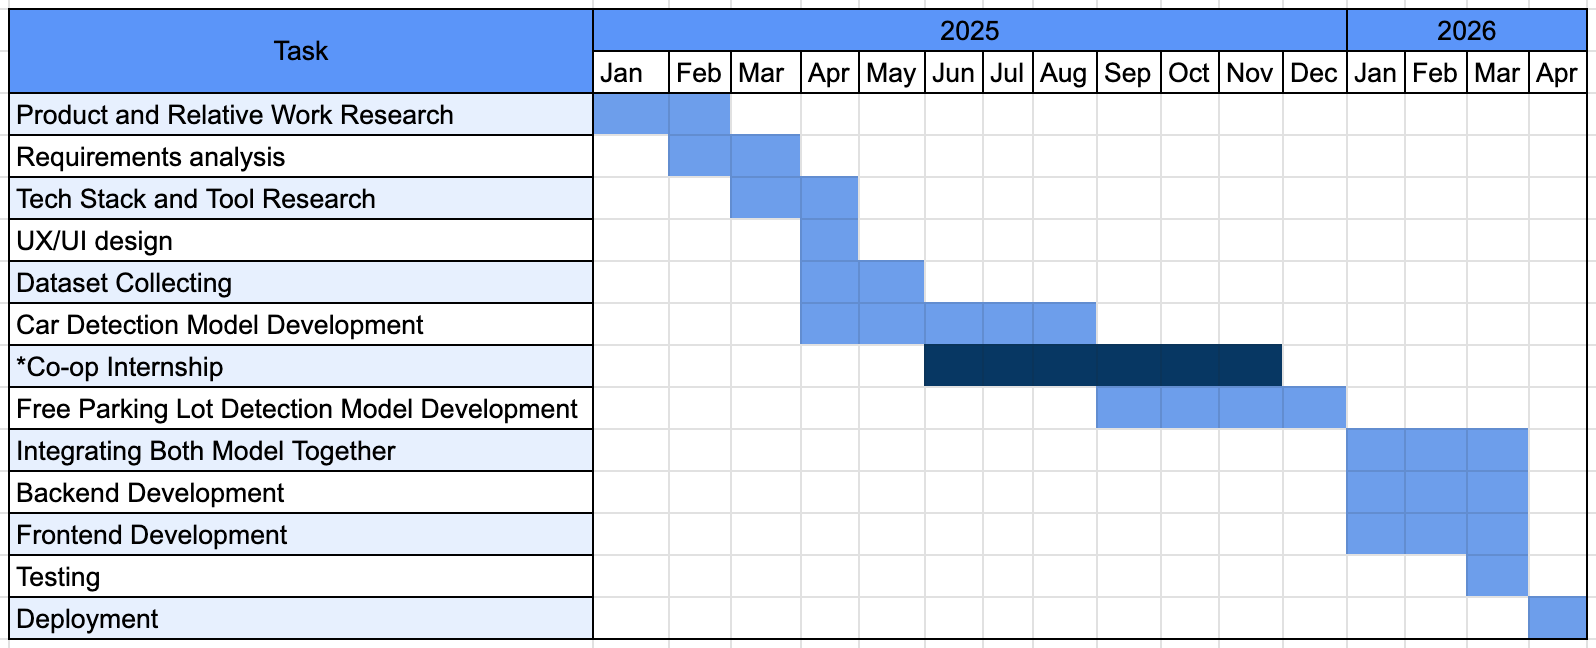
\includegraphics[width=\textwidth,height=0.5\textheight,keepaspectratio]{timeline/KU-Parking_timeline.png}
    \caption{Proposed Timeline for KU Parking Project}
    \label{fig:timeline-dev-progress}
\end{figure}

\section{Modules Developed}
\label{section:module-developed}
<Test Modules Developed>

\section{Screenshot}
\label{section:screenshot}
<Test Screenshot>


\section{Experimental Results}
\label{section:experimental-results}
<Test Experimental Results>

\section{Datasets}
\label{section:datasets}
We've modified our dataset collection method. Due to the semester break in mid-April, footages captured from the Computer Department Parking Facility contained a limited number of cars, resulting in a less diverse dataset. To improve the variety and robustness of our car detection dataset, we supplemented it with online footage sources to our train dataset.

For dataset we've used to train, visit Google Drive: \url{https://drive.google.com/drive/folders/1pOUgcbsFb1mpLc5oywZ2xQdRepm_nVu7?usp=sharing}

\section{Gantt chart}
\label{section:gantt-chart}
As of May 11, 2025, the current timeline for the KU Parking Project is depicted in Figure \ref{fig:11-05-25-timeline-dev-progress}.
\begin{figure}[h!]
    \centering
    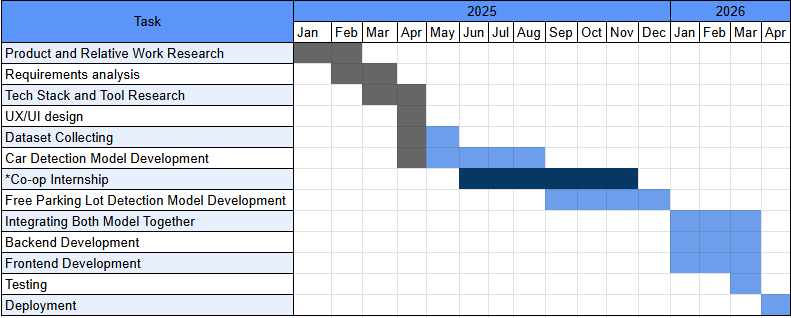
\includegraphics[width=\textwidth,height=0.5\textheight,keepaspectratio]{timeline/11-05-25-KU-Parking-timeline.PNG}
    \caption{Updated Timeline for KU Parking Project}
    \label{fig:11-05-25-timeline-dev-progress}
\end{figure}

\section{Self-evaluation}
\label{section:self-evaluation}
As mentioned in the Datasets section (Section \ref{section:datasets}), we have modified our dataset collection approach. This has led to minor adjustments and re-planning during the data collection phase. Model development remains on schedule; however, we anticipate that the upcoming Cooperative Internship period, spanning from June to November, may affect the development pace. Consequently, further development of the Parking Lot Detection Model may be postponed to January 2026. In the worst-case scenario—if the Car Detection Model is not completed before the end of January 2026—we may need to consider cutting the Parking Lot Detection Model and shifting focus to software-side development.